%!TEX root = ../Main.tex

\chapter{Exercise 7}

In this exercise, a custom IP called "advios" is created using SystemC. Then a test-bench is written that verifies the functionality of the IP. Using the tool "vivado HLS", the C-code is synthesized into VHDL-code. Using the aforementioned test-bench, the VHDL-code is verified to have the same funcitonlaity as the C-code.
After synthesizing the IP, a project is created, in which the IP is used in an application, and the functionality is tested through visual inspection.

\begin{figure}[b]
	\centering
	{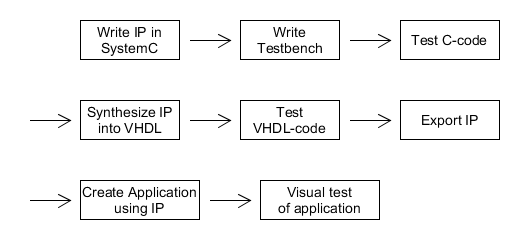
\includegraphics[scale=0.5]{Images/2_7_procedure.png}}\\[0.5cm]
	\label{fig:7_procedure}
	\caption{Procedure of exercise 7.}
\end{figure}

\FloatBarrier

\section{Implementation of IP using SystemC}
First, the IP is implemented using SystemC. The interfaces and the functionality is given in the assignment, as seen in figures \ref{fig:7_block} and \ref{fig:7_functionality}.

\begin{figure}[b]
	\centering
	{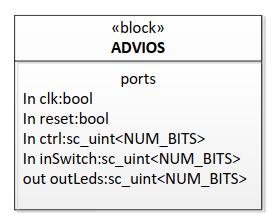
\includegraphics[scale=0.5]{Images/2_7_block.png}}\\[0.5cm]
	\label{fig:7_block}
	\caption{Procedure of exercise 7.}
\end{figure}
\begin{figure}[b]
	\centering
	{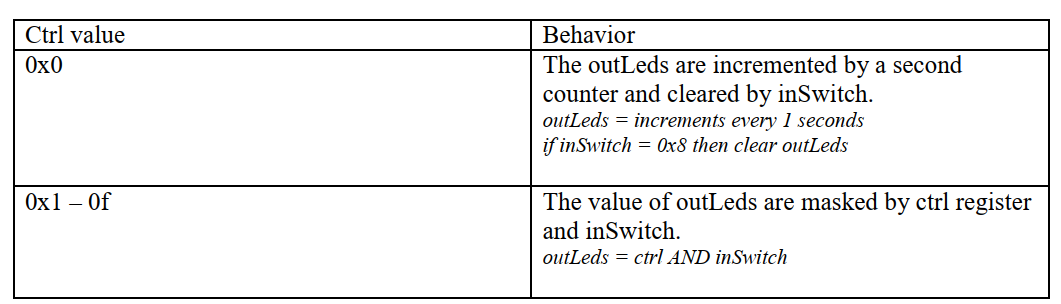
\includegraphics[scale=0.5]{Images/2_7_functionality.png}}\\[0.5cm]
	\label{fig:7_functionality}
	\caption{Procedure of exercise 7.}
\end{figure}

\FloatBarrier

The IP is implemented in the following .h and .cpp-files.

 \begin{lstlisting}
 #pragma once
 #include <systemc.h>
 
 #define NUM_BITS 4
 #define CLKFREQ = 100000000 
 
 #ifndef _ADVIOS_
 #define _ADVIOS_
 
 #include <systemc.h>
 
 SC_MODULE(advios) {
 
 //Ports
 sc_in <bool> clk;
 sc_in <bool> reset;
 sc_in<sc_uint<NUM_BITS> > ctrl;
 sc_in<sc_uint<NUM_BITS> > inSwitch;
 sc_out<sc_uint<NUM_BITS> > outLeds;
 
 // Signal to communicate between the two threads.
 sc_signal<bool> oneSecPulse;
 
 //Variables
 sc_uint<8> switchs;
 
 int clkCount; // Used in clock-divider-thread
 
 //Process Declaration
 void adviosThread();
 void clkDivide();
 void writeToLeds();
 
 //Constructor
 SC_CTOR(advios) {
 clkCount = 0;
 //Process Registration
 // Clock-divider-thread, which outputs a high signal to oneSecPulse once every second.
 SC_CTHREAD(clkDivide, clk.pos());
 reset_signal_is(reset, true);
 
 // "Main"-thread for the module.
 SC_CTHREAD(adviosThread, clk.pos());
 }
 };
 
 #endif
 \end{lstlisting}
 \label{lst:advios_h}
 
 \begin{lstlisting}
 #include "Advios.h"
 
 void advios::clkDivide()
 {
 while (1)
 {
 // Clock = 100 MHZ.
 // Every 100*1000*1000 cycles, make a "true" pulse, and reset the counter.
 clkCount++;
 if (clkCount >= 100000000)
 {
 oneSecPulse.write(true);
 clkCount = 0;
 }
 else
 {
 oneSecPulse.write(false);
 }
 // Wait to be triggered by clock again.
 wait();
 }
 }
 
 void advios::adviosThread()
 {
 
 // Used in connecting the ctrl-port to the AXI4Lite-interface.
 #pragma HLS resource core=AXI4LiteS metadata="-bus_bundle slv0" variable=ctrl
 
 // Init counter
 sc_uint<4> cnt = 0;
 
 while (1)
 {
 // if ctrl == 0, write value of counter to LEDs. Counter increments 1 every second.
 // if ctrl != 0, write the value of the switches masked by the ctrl-signal.
 int val_ctrl = ctrl.read().to_int();
 int val_switches = inSwitch.read().to_int();
 if (val_ctrl == 0)
 {
 outLeds.write(cnt);
 // if all switches are engaged, clear LEDs and reset counter.
 if (val_switches == 0x8)
 {
 outLeds.write(0);
 cnt = 0;
 }
 else
 {
 // If the one-sec-pulse is high (which it is for only 1 cycle pr. second), increment the counter.
 if (oneSecPulse == true)
 {
 //Increment counter, write to LEDs and wait for new clock.
 cnt++;
 outLeds.write(cnt);
 }
 }
 }
 else
 {
 //	sc_uint<NUM_BITS> outLedVal = val_switches && val_ctrl;
 outLeds.write((val_switches & val_ctrl));
 }
 
 // Wait to be triggered by clock again.
 wait();
 }
 }
 
\end{lstlisting}
\label{lst:advios_cpp}

\section{Test of C-code}
In order to test the functionality of the C-code, a test-bench and a driver is made.
The driver defines the interfaces to the "Device Under Test", along with a series of input stimuli and expected outputs. The test-bench sets up the test environment and executes the test-simulation.

The drivers and the test-bench are implemented in the following .h and .cpp-files
\begin{lstlisting}
#ifndef _ADVIOS_DRIVER
#define _ADVIOS_DRIVER

#include <systemc.h>
//#include "Advios.h"

#define NUM_BITS 4

SC_MODULE(advios_driver) {

//Ports
sc_in <bool> clk;
sc_out <bool> reset;

sc_out<sc_uint<NUM_BITS> > ctrl;
sc_out<sc_uint<NUM_BITS> > outSwitch;
sc_in<sc_uint<NUM_BITS> > inLeds;

int retval;

//Process Declaration
void test();

//Constructor
SC_CTOR(advios_driver) : retval(-1) {

//Process Registration
SC_THREAD(test);
sensitive << clk.pos();
}
};

#endif
\end{lstlisting}
\label{lst:advios_driver_h}

\begin{lstlisting}
#include "advios_driver.h"

void advios_driver::test() {


//Variables
sc_uint<NUM_BITS> sw_test;
sc_uint<NUM_BITS> ctrl_test;
sc_uint<NUM_BITS> led_result;

//Initialization
sw_test = 0b1111;
ctrl_test = 0b0111;

// Reset at start, then make sure reset is false.
reset.write(true);
wait();
reset.write(false);
wait();

// Write stimuli to DUT
ctrl.write(ctrl_test);
outSwitch.write(sw_test);

// Wait for DUT to react to stimuli.
wait();
wait();

// Record output
led_result = inLeds.read();
wait();

// Compare output to expected value.
if (ctrl_test == led_result)
retval = 0;
else
retval = 1;
}
\end{lstlisting}
\label{lst:advios_driver_cpp}

\begin{lstlisting}
#include <systemc.h>
#include <stdio.h>

// if running RTL-simulation use generated RTL-wrapper
#ifdef __RTL_SIMULATION__
#include "advios_rtl_wrapper.h"
#define advios advios_rtl_wrapper
// if not, the c-simulation is being run, and the c-version is used instead.
#else
#include "advios.h"
#endif

#include "advios_driver.h"

#define TRACE_FILE_NAME "advios_trace"

int sc_main (int argc , char *argv[])
{
sc_report_handler::set_actions("/IEEE_Std_1666/deprecated", SC_DO_NOTHING);
sc_report_handler::set_actions( SC_ID_LOGIC_X_TO_BOOL_, SC_LOG);
sc_report_handler::set_actions( SC_ID_VECTOR_CONTAINS_LOGIC_VALUE_, SC_LOG);
sc_report_handler::set_actions( SC_ID_OBJECT_EXISTS_, SC_LOG);

sc_trace_file *tracefile;

// Test signals
sc_signal<bool> s_reset;
sc_signal<sc_uint<NUM_BITS> > s_switch;
sc_signal<sc_uint<NUM_BITS> > s_ctrl;
sc_signal<sc_uint<NUM_BITS> > s_leds;

// Create a 10ns period clock signal
sc_clock s_clk("s_clk", 10, SC_NS);
advios U_Advios("advios");
advios_driver U_advios_driver("advios_driver");

// Create tacefile
tracefile = sc_create_vcd_trace_file(TRACE_FILE_NAME);
if (!tracefile) cout << "Could not create trace file." << endl;

// Set resolution of trace file to be in 10 US
tracefile->set_time_unit(1, SC_NS);

// Trace signals
sc_trace(tracefile, s_clk,    "clock");
sc_trace(tracefile, s_reset,  "reset");
sc_trace(tracefile, s_ctrl,   "ctrl");
sc_trace(tracefile, s_leds,   "leds");
sc_trace(tracefile, s_switch, "switch");

// Connect the DUT to the signals
U_Advios.clk(s_clk);
U_Advios.reset(s_reset);
U_Advios.ctrl(s_ctrl);
U_Advios.outLeds(s_leds);
U_Advios.inSwitch(s_switch);

// Connect the driver to the signals
U_advios_driver.clk(s_clk);
U_advios_driver.reset(s_reset);
U_advios_driver.inLeds(s_leds);
U_advios_driver.outSwitch(s_switch);
U_advios_driver.ctrl(s_ctrl);

// Simulate for 200
int end_time = 200;
std::cout << "INFO: Simulating" << std::endl;
// start simulation
sc_start(end_time, SC_NS);

// Check whether test passed or not
if (U_advios_driver.retval == 0) {
printf("Test passed !\n");
} else {
printf("Test failed !!!\n");
}

// Close trace file.
sc_close_vcd_trace_file(tracefile);
std::cout << TRACE_FILE_NAME << ".vcd" << std::endl;

return U_advios_driver.retval;
};

 \end{lstlisting}
\label{lst:tb_advios}

\subsection{Result of C-simulation}
Figure \ref{fig:7_csim} show the result of running the C-simulation of the code. As seen, the test is passed, which indicates that the received result from the simulated matched the expected result.
\begin{figure}[b]
	\centering
	{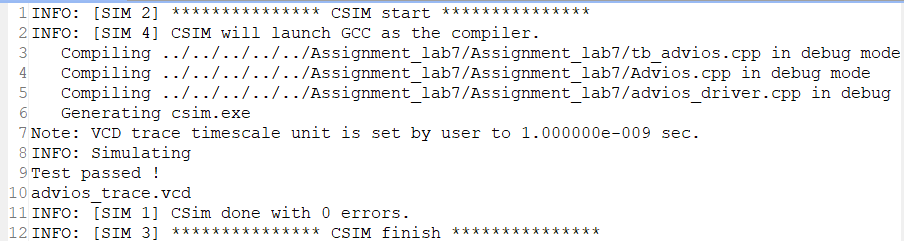
\includegraphics[scale=0.5]{Images/2_7_csim.png}}\\[0.5cm]
	\label{fig:7_csim}
	\caption{Result of C-simulation}
\end{figure}

\section{Synthesis of C-code into VHDL}
Using Vivado HLS, the C-code is synthesized into VHDL-code. From the figures \ref{fig:7_synth_performance} and \ref{fig:7_synth_utilization} the performance and resource utilization of the synthesized code can be seen. It can be seen that there is a latency of a maximum of 5 clock cycles throughout the module. Furthermore, it can be seen that there is only used 170 Flip Flops and 187 Lookup Tables, which is virtually none of the existing resources of the board.
\begin{figure}[b]
	\centering
	{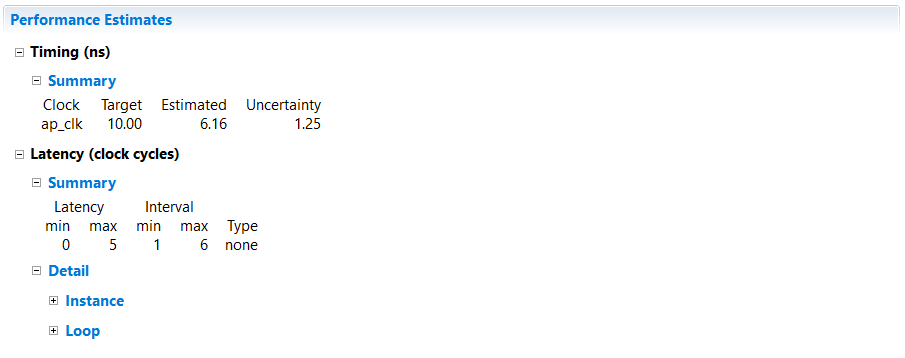
\includegraphics[scale=0.5]{Images/7_synth_performance.png}}\\[0.5cm]
	\label{fig:7_synth_performance}
	\caption{Performance of synthesized VHDL code.}
\end{figure}
\begin{figure}[b]
	\centering
	{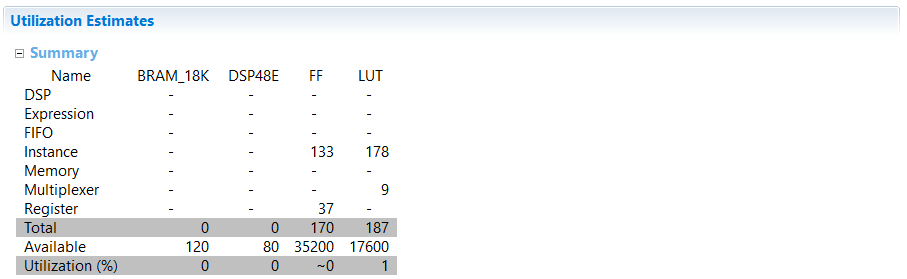
\includegraphics[scale=0.5]{Images/7_synth_utilization.png}}\\[0.5cm]
	\label{fig:7_synth_utilization}
	\caption{Resource utilization of synthesized VHDL code.}
\end{figure}

\FloatBarrier

\section{RTL/C co-simulation}
In order to verify that the synthesized VHDL-code functions as expected, an RTL/C co-simulation is carried out. Basically, a the test defined using the test bench and the driver is carried out, first on C-level as before, and then again using the newly synthesized VHDL-code. It then compares the result of the two tests, in order to verify that the functionality is the same.

As seen in figure \ref{fig:7_cosim_res}, it is seen that the simulation passes, indicating that the functionality of the synthesized VHDL-code matches that of the C-code.

\begin{figure}[b]
	\centering
	{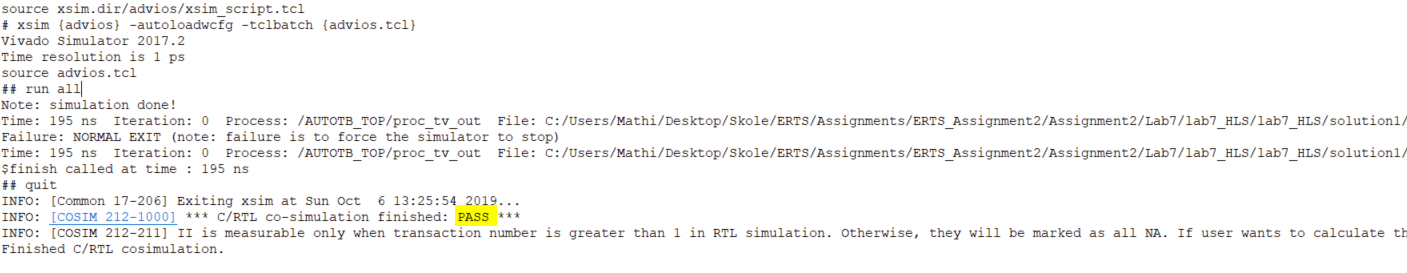
\includegraphics[scale=0.5]{Images/2_7_cosim_res.png}}\\[0.5cm]
	\label{fig:7_cosim_res}
	\caption{Result of RTL/C co-simulation}
\end{figure}

\section{Connect ctrl-port to AXI4Lite-interface}
The ctrl-port is connected to the AXI4Lite-interface, simply by adding the following line of code

\begin{lstlisting}
	#pragma HLS resource core=AXI4LiteS metadata="-bus_bundle slv0" variable=ctrl
\end{lstlisting}
at the top of the "main"-thread of the advios-module, as seen in the file Advios.cpp.
This makes it possible to connect an external signal to the block in order to send messages to the ctrl-port of the module.

\section{Using the IP in an application}
\subsection{Generating the hardware}
After having exported the RTL core from Vivado HLS, by simply pressing "Export RTL", the IP core can be used in a Vivado block design. A design was made using the IP, the ZYNQ processing system and an instance of the AXI4Lite-interface, as seen in figure \ref{fig:2_7_BD}.

\begin{figure}[b]
\centering
{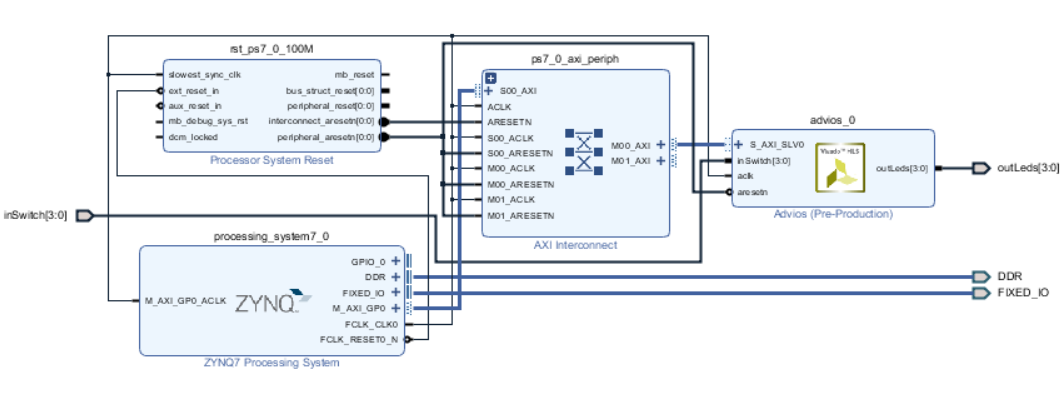
\includegraphics[scale=0.5]{Images/2_7_bd.png}}\\[0.5cm]
\label{fig:2_7_BD}
\caption{Block design using the exported IP.}
\end{figure}

Next, the bitstream is generated, and the hardware is exported to Xilinx SDK, where an application for the hardware is written.

\subsection{Writing the application}
A simple application is written, which uses UART-communication to promt the user for a value to be used as the ctrl-value. Upon receiving a new value, the value is written to the ctrl-signal. As the rest of the functionality is handled by hardware, the program will function as expected, even though the "main"-program is waiting for a new input from the user.

\begin{lstlisting}
#include "xparameters.h"
#include "xadvios.h" // Include HAL for iosc driver
//====================================================
void writeToCtrl(int);

// driver created as global, so it can be used in "helper"-funciton writeToCtrl.
XAdvios adviosHLS; // Create an instance of the advios driver

int main (void)
{
// Initialize the advios driver
if (XAdvios_Initialize(&adviosHLS, XPAR_ADVIOS_0_DEVICE_ID) != XST_SUCCESS) return XST_FAILURE;

xil_printf("-- Start of the Program --\r\n");

// Loop: Prompt user for ctrl-value. If valid value, write to ctrl, else tell user.
while(1)
{
xil_printf("\r\n");
xil_printf("-------------------------------\r\n");
xil_printf("\r\n");
xil_printf("Enter ctrl-value\r\n");

int userInput = inbyte()-48;
if ((userInput <0 )||(userInput > 15))
{
xil_printf("Value must be between 0 and 15\r\n");
}
else
{
writeToCtrl(userInput);
}
}
}


void writeToCtrl(int val)
{
// Writing 0xff to the ctrl register of the iosc IP core
XAdvios_SetCtrl(&adviosHLS, val);
}
\end{lstlisting}
\subsection{Results}
Upon visual inspection, the following functionality is confirmed:
\begin{itemize}
	\item \textbf{ctrl = 0:} The LEDs are used to count, incrementing with the value of 1 every second.
	\item \textbf{ctrl = 1-15:} The LEDs show the value of the number corresponding to the value of ctrl, provided that all switches are in the "on"-position. If a switch is in the "off"-position, the corresponding LED is turned off. 
\end{itemize}

Thus, the functionality of the system is as stated in the requirements.

\section{Summary}
In this exercise, an IP has been written in C using SystemC, synthesized using High Level Synthesis, and integrated in a design. It has taught us the general procedure for creating custom IPs at a relatively high level of abstraction, in order to utilize them at a much lower level of abstraction.